\chapter{GRAIN PHYSICS}
% !TEX root = hazy3.tex

\section{Overview}

The following discussion outlines some physical processes relating to
grains, as incorporated in \Cloudy.  It is adopted from \citet{Baldwin1991},
and was written in close collaboration with P.G. Martin.

Much of this physics has been updated to that described by \citet{VanHoof2004}, which is based on \citep{Weingartner2001a}.

Several grain populations, types of graphite and ``astronomical
silicates'', are available.  Usually one of each type, for a total of two,
is selected, although there is no limit to the number of grain populations.
Optical properties like opacity of the species are based on a realistic
power-law size distribution.  Other properties (like potential and
temperature) are computed for a mean grain size rather than calculated for
each individual size.

 The following describes the ``old'', default, grains that were originally
incorporated into the code in the late 1980's (\citealp{Baldwin1991}).  These
use optical properties that correspond to averages over the grain size
distribution.  The current treatment both resolves the grain
size distribution and includes single photon heating for the smaller grains.
This new treatment is described in \citet{VanHoof2001} and will be
included in this document at a later time.

\section{Grain opacity}

Grains are not included in the calculation by default.  When enabled
with the grain command the default mixture has interstellar medium (ISM)
properties.  Grains more similar to those seen in Orion or planetary nebulae
are also available.

\subsection{ISM grains}

The optical constants for the default (ISM) grain species are from the
calculations of \citep{Martin1990}.  These extend the work of
\citep{Draine1984} to ionizing energies where the grains are strongly absorbing.
These opacity calculations were based on the
\citep{Mathis1977} power-law size distribution to simulate interstellar extinction in
diffuse clouds.

\subsection{Orion grains}

Grains within the Orion Nebula have a relatively large ratio of total
to selective extinction $R$ and an exceptionally gray opacity in the
ultraviolet.  These are both indicative of a deficiency in small grains
and a larger mean grain size.  To account for this, a second set of opacity
functions is included, the Orion group.  For this the value of the smallest
size (a$_-$) in the \citep{Mathis1977} size distribution was increased from
0.0025$\mu$m to 0.03$\mu$m.  While this simple adjustment of the size distribution
is not entirely adequate for explaining the details of the visible and near
ultraviolet Orion extinction curve \citep{Mathis1981}, it should
be an improvement for the ionizing ultraviolet portion, which is most
important.

The Orion extinction curve is designed to simulate the large R grains
observed in this H~II region.  Relative to ISM standard grains the total
amount of grain material was preserved, so that $\alpha_{\mathrm{abs}}$ in the infrared and
in the EUV and X-Ray regions remains unchanged.  The main differential effect
is to lower the cross section through a broad peak at 1 Ryd.

\subsection{PN grains}

Infrared opacities for the silicate component are taken from unpublished
work by K. Volk.  Ultraviolet silicate cross sections, and the graphite
constituent, are standard ISM.

\subsection{Extinction}

The ISM extinction properties, both effective scattering (subscript scat)
and absorption (subscript abs), are shown in Figure~\ref{fig:GrainOpacity}.

\begin{figure}
\centering
\label{fig:GrainOpacity}
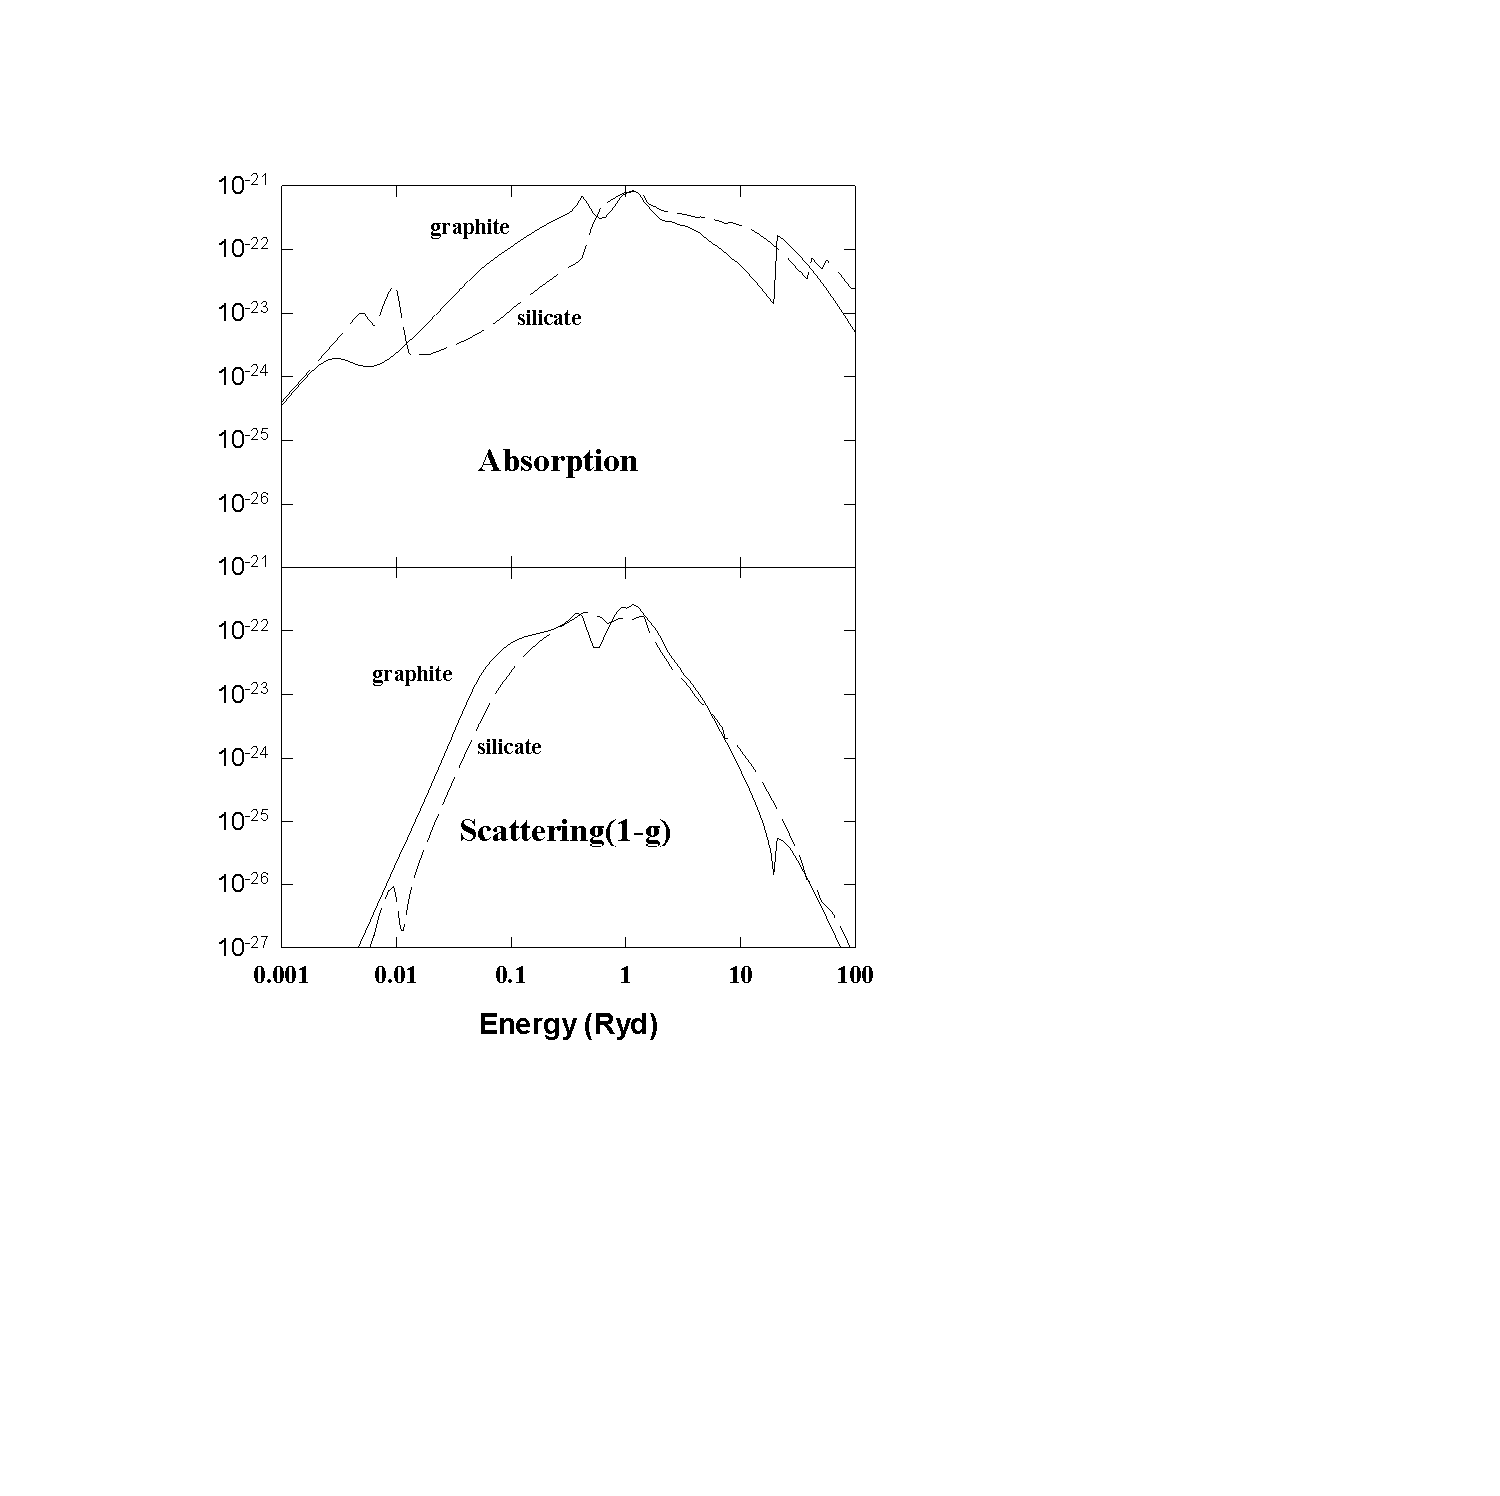
\includegraphics{GrainOpacity}
\caption[Grain opacities]{The absorption and scattering cross sections (cm$^2$ per hydrogen
nucleon) for the two ISM grain populations, graphite and silicate, are shown.
The effective scattering cross section is the scattering cross section
multiplied by $1-g$, where $g$ is the asymmetry parameter.}
\end{figure}

The quantities plotted are cross sections (cm$^2$) per H nucleon:
$\sigma = \kappa/n(H)$,
where $\kappa$ (cm$^{-1}$) is the opacity due to grains and $n(H)$
(cm$^{-3}$) is the local
density of H in any form.  Rather than the total scattering cross section
$\sigma_s$ an effective scattering cross section $\sigma_{scat} = \sigma_s
(1-g)$ is plotted.  This
discounts the radiation scattered near the forward direction.  The asymmetry
parameter $g$ approaches unity at high and low energies, particularly for
larger grains, so that $\sigma_{scat}$ becomes much less than $\alpha_{abs}$

The optical depth $\tau$ is $\sigma$ times the hydrogen column density
(or $\kappa$ integrated
over the path).  Absorption attenuates the incident radiation field as
exp($-\tau_{abs}$).  The effects of scattering are more difficult to model.  In an
open geometry, scattering attenuates approximately as
$(1+0.5 \tau_{scat})^{-1}$.
However, in a closed geometry, to within factors of order unity, the
scattered light is not lost from the beam, and the scattering opacity can
be ignored.  In either case, effective grain scattering optical depth is
generally fairly small through the ionized nebula at ionizing energies.

\section{Photoelectric emission}

As discussed below, photoelectric emission from grains contributes
directly to heating the gas and, through the grain potential U$_g$ established,
affects radiative and collisional heating of the grains and the grain drift
velocity.

The photoionization rate of a grain, per unit projected area, is
\begin{equation}
{\Gamma _g} = \int_{{\nu _o}}^\infty  {{Q_{abs}}\frac{{4\pi J}}{{h\nu
}}\,\hat Y} \;d\nu
\end{equation}
where $\hat Y$ is the effective photoelectric yield per absorbed photon,
$Q_{abs}$ is the
absorption efficiency factor, and $4 \pi J/h\nu$ symbolizes the photon flux of
direct, diffuse, and OTS radiation fields.  For the OTS line component,
the integral is of course just a sum over the line photons that are
sufficiently energetic.  The threshold for photoemission, to be determined
self-consistently, is given by $h\nu_o = \max\{V_n+V_g, V_n\}$, where $V_n$ is the
photoelectric threshold for a neutral grain and $V_g = eU_g$.

$V_g$ will depend on grain size through $Q_{abs}$ and $\hat Y$.  In the
present implementation, a typical $V_g$ is defined for each species
by using Qabs averaged over the size distribution: $Q_{abs} =
\alpha_{abs}/\Sigma = \kappa_{abs}/n(H)\Sigma$.  The projected grain area
per H, $\Sigma$, is similar for each species: $2.1 \times 10^{-22}$
cm$^2$ for graphite and $2.4 \times 10^{-22}$ cm$^2$ for silicates.

$\hat Y$ is constructed as follows.
The basic laboratory data measure the yield
(per absorbed photon) for a neutral surface, $Y_n$.
For each incident photon
energy $h\nu$, the photoelectrons emerging from the neutral surface have varying
energies $E$, with a probability distribution $p_n(E)$.
To account for electron
escape from finite sized
grains, yields measured for semi-infinite sheets in the laboratory have
to be corrected by a factor $f(E)$ (which introduces a size dependence).
Such a correction would change the shape of the probability distribution
as well as increase the integrated emission from a neutral surface (\citealp{Draine1978} gives an approximate expression for the overall increase).  Then,
formally
\begin{equation}
\hat Y = {Y_n}\int_{{E_o}}^{\left( {h\nu  - {V_n}} \right)} {f\,{p_n}\;dE}
\end{equation}
where $E_0 = \max\{0 , V_g\}$ introduces the fact that the lowest energy
photoelectrons do not escape from positively charged grains.

The form adopted is
\begin{equation}
{Y_n} = \min \left\{ {{Y_o}\left( {1 - {V_n}/h\nu } \right),{Y_1}}
\right\}
\end{equation}
for $h\nu\ge  V_n$, and $V_n = 8$ eV and $Y_0 = 0.5$ is assumed for both grain populations;
according to \citet{Draine1978} this combination gives about the right amount
of photoelectric emission to heat neutral H I clouds in interstellar space
$(h\nu \le 13.6$ eV).  For the higher energies a cap at $Y_1 = 0.2$ is introduced,
which is suggested by experimental data.  For $p_n$ a simple form that is
independent of $E$ (\citealp{Draine1978}) is adopted:
\begin{equation}
{p_n} = {\left( {h\nu  - {V_n}} \right)^{ - 1}}\quad .
\end{equation}

While only approximate, this induces the physically correct response
(decrease) in $\hat Y$
(and the photoelectric heating) when the grain is positively charged.
Because the form of $f(E)$ is highly uncertain $f = 1$ is assumed (this again
avoids a size dependency).
Extension of the flat cap in $Y_n$ to high energies
also addresses this issue to some degree.
With these assumptions,
${\mathrm{\hat Y}}$
is known in analytic form:
\begin{equation}
\hat Y = {Y_n}\min \left\{ {1,\;1 - {V_g}/\left( {h\nu  - {V_n}} \right)}
\right\}\;.
\end{equation}

\section{Collisional charging of a grain}

Per unit projected area of a grain, collisions with particles of space
density $n$, mass $m$, and charge $Z$ $(Z = -1$ for electrons) give an effective
recombination rate
\begin{equation}
\alpha \left( {gr} \right) =  - n\;\bar v\;SZ\;\eta \;,
\end{equation}
where
\begin{equation}
\bar v = \sqrt {8kT/\pi \,{m_e}}
\end{equation}
is the mean particle speed.  In this expression, and for other collisional
rates involving $n$ below, it is implicit that there is a sum of similar terms
over all species in the gas.  For electrons $S$ is the sticking probability
which we take to be 1 (\citealp{Spitzer1948}; \citealp{Watson1972}; \citealp{Draine1978}).  For
positively charged nuclei, $SZ$ is the charge transfer efficiency, taken to
be $Z$ here.  The last factor $\nu$, the correction for Coulomb interactions between
the grain and the recombining particles of charge $Z$, is given in terms of
\begin{equation}
\psi  = Z{V_g}/k{T_e}
\end{equation}
by
\begin{equation}
\eta  = \left\{ {\begin{array}{*{20}{c}}
   {1 - \psi } \& {if} \& {\psi  \le 0}  \\
   {\exp \left( { - \psi } \right)} \& {if} \& {\psi  > 0}  \\
\end{array}} \right.
\end{equation}
Terms for positively charged nuclei are included, but are usually small
relative to the contribution from free electrons.

\section{Grain potential}

The steady state grain potential is determined for each grain species
independently by requiring charge balance.  Expressed as a balance per unit
area this is $\alpha_{gr} = \Gamma_{gr}$. Because of the many dependencies
on $V_g$, this is carried
out numerically.

\section{Grain drift velocity}

The grain drift velocity is determined by balancing the radiative
acceleration due to the direct attenuated radiation field with the drag
forces given by equations 1--6 of \citet{Draine1979}.  The equations
are solved numerically for the drift velocity, including interactions with
electrons and all ions present in the gas.

\section{Radiative heating and cooling of a grain}

Once the grain potential is known, the rate of radiative heating of the
grain per unit projected area is
\begin{equation}
{G_{grain}}(rad) = \int_0^{{\nu _o}} {{Q_{abs}}4\pi \,J\;d\nu  + \int_{{\nu
_o}}^\infty  {{Q_{abs}}\frac{{4\pi J}}{{h\nu }}\;\left( {h\nu  - EY} \right)}
} \;d\nu \;.
\end{equation}
The last term represents the portion of the photon energy that does not
heat the grain, but rather passes to the escaping electrons:
\begin{equation}
EY = {Y_n}\int_{{E_o}}^{\left( {h\nu  - {V_n}} \right)}
{E\;f\,{p_n}\;dE\quad .}
\end{equation}
With the above approximations for $f$ and $p_n$ this is given analytically by
\begin{equation}
EY = 0.5\;{Y_n}\;\left[ {{{\left( {h\nu  - {V_n}} \right)}^2} - {{[\max
(0,{V_g})]}^2}} \right]/\left( {h\nu  - {V_n}} \right)
\end{equation}

The cooling of a grain by radiative losses, per unit projected area,
is given by
\begin{equation}
{\Lambda _{grain}}\left( {rad} \right) = \int_0^\infty  {{Q_{abs}}\;4\pi
\,{B_\nu }\left( {{T_g}} \right)\;d\nu }
\end{equation}
where $B_\nu(T_g)$ is the Planck function for the grain temperature.

\section{Collisional heating of a grain}

Collisions with electrons, ions, and neutral particles also heat the
grains.  Per unit projected area of the grain, this heating rate may be
written as
\begin{equation}
{G_{grain}}\left( {col} \right) = n\;\bar v\;S\;\left( {2k{T_e}\xi  -
Z{V_g}\eta  + I\,\eta  - 2k{T_g}\,\eta } \right).
\end{equation}
The first term corresponds to kinetic energy extracted from the gas.  The
factor  makes adjustment for Coulomb interactions and is given by
\begin{equation}
\xi  = \left\{ {\begin{array}{*{20}{c}}
   {1 - \psi /2} \& {if} \& {\psi  \le 0}  \\
   {\left( {1 + \psi /2} \right)\exp \left( { - \psi } \right)} \& {if}
\& {\psi  > 0}  \\
\end{array}} \right..
\end{equation}
The second term in $G_{grain}(col)$ allows for the change of the particle's energy
in the grain potential.  In the third term, the product $I\eta$ is the average
chemical energy released per impact.  Here it is assumed that when impinging
ions recombine the ionization energy released is deposited as heat in the
grain (there is then no corresponding term for heating the gas in
$\Lambda_g$ below).
The last term describes the effect of thermal evaporation of neutralized
ions and thermally accommodated neutral particles (there is no corresponding
term for electrons).

In implementing the above processes, $S$ for electrons is again the sticking
probability.  For positively charged nuclei, $S$ is the energy transfer
efficiency, taken here to be unity (this process should be evaluated
consistently with that for charge transfer).  For neutral particles of mass
$m$ striking a grain whose typical atom has mass $M$, the accommodation
coefficient $S \approx 2 m M/(m + M)^2$ (\citealp{Draine1978}).

\section{Grain temperature}

The equilibrium grain temperature is determined by the balance between
cooling $(\Lambda)$ and heating $(G)$ by radiative and collisional processes.  For
the radiative terms, $Q_{abs}$ averaged over the size distribution is used to
obtain a typical temperature for each species.

As a test of the bandwidth of the code, and its behavior in a well-defined
limit, tests where computed in which the grains were irradiated by black
body radiation in strict thermodynamic equilibrium (i.e., the color and
energy density temperatures were equal).  Radiation temperatures between
10 K and 10$^9$~K, the temperature limits to the code, were used.  These tests
showed that the deduced grain equilibrium temperature was within much better
than 1 percent of the blackbody temperature.

\section{Photoelectric heating of the gas}

Heating of the gas by photoemission from grains can be an important
process in ionized regions (\citealp{Spitzer1948};
\citealp{Oliveira1986}).  For
charged grains this heating rate (erg cm$^{-3}$ s$^{-1}$) is given by
\begin{equation}
{G_{gas}} = \int_{{\nu _o}}^\infty  {{\kappa _{abs}}\frac{{4\pi J}}{{h\nu
}}\;\left( {EY - {V_g}\hat Y} \right)\;d\,\nu \;.}
\end{equation}
The first term describes the energy of the photoelectrons as they leave
the surface, balancing the similar term in $G_{grain}(rad)$.  The second term
compensates for the grain potential, and can be seen to balance the related
term in $G_g(col)$ when charge balance holds.

\section{Collisional cooling of the gas}

The gas is cooled as the gas particles hit the cooler grain surface.
Per unit volume, this cooling rate may be written as
\begin{equation}
{\Lambda _{gas}} = n\;n(H)\;\Sigma \,\bar v\;S\,\left( {2k{T_e}\xi  -
2k{T_{grain}}\eta } \right),
\end{equation}
the individual terms consistently balancing the corresponding ones in
$G_g(col)$.

\section{Grain sublimation}

The code checks that grain survival is likely by comparing the highest
grain temperature with the sublimation temperatures.  These are taken to
be 1400 K for silicates and 1750 K for graphite and are based on the paper
by \citet{Laor1993}.  A warning will be printed at the
end of the calculation if the grain temperature rises above the sublimation
point.  A caution will be printed if the temperature rises above 90\% of
the sublimation point.

\section{Ionic recombination on grain surfaces}

Positive ion recombination on grain surfaces proceeds at a rate
$n_{ion}n_H\alpha_{gr}$
where the recombination coefficient is taken from \citet{Draine1987};
their equation 5.15).  For a standard grain size distribution this rate
coefficient is $\sim 5.8\times 10^{-13}T_e^{-0.5}$ cm$^3$ s$^{-1}$.  This process is included for
all ions included in the calculation when grains are present, but is not
generally important.
